%%% Local Variables:
%%% mode: latex
%%% TeX-master: t
%%% End:

% !Mode:: "TeX:UTF-8"

\chapter{MPSoC结构级热分析算法的验证实验}
\label{cha:SSTAexperiments}

\section{验证实验平台}
本文选择热分析软件HotSpot(版本5.02)作为验证基准,构建3个测例进行温度-功耗数据对比分析, 从而检验所提出的模块级、核级、改良核级这3种热分析方法的精度与效率。HotSpot软件以及三种热分析方法的运行平台为为配有Intel酷睿i7,8G 内存,运行Ubuntu 10.04 LTS操作系统的PC机。

\section{验证实验所用到的测例}
测例1采用文献\onlinecite{LrnAutoRegMdlFstTransThemAlysCp}策略,将4个Alpha21264核心组合为一个4核处理器。 每个Alpha21264的处理核心核配有两块独享缓存L2\_Right、L2\_Left,4个核共享最后一级缓存L3。 芯片的布局为:将处理核心放置于芯片的四个角落,每个核的独享缓存处于核的周围, 而将共享缓存区置于芯片中心(这样做不仅考虑了处理单元的片上散热问题, 也有利于通过功率较低的共享缓存,隔断功率较大的多个核相互之间的热交换影响)。

测例2采用Intel Sandy Bridge-E架构的8核高端CPU芯片\onlinecite{INTELi7}。 近似正方形的i7-3960X芯片核心面积为435$mm^2$(长宽尺寸分别为20.9$mm^2$、20.8$mm^2$)。本文中,我们按照Sandy Bridge-E i7-3960X的布局原则模拟生成了一种较为简略的芯片布局结构,整体平面图如图\ref{fig:core-i7-flp}所示, 主要具有的模块为:双精度数据输入输出模块(DDR IO),最后一级缓存模块(LLC),核心模块,快速互联通道模块(QPI), 外设成员互联通道模块(PCI-E),功耗控制单元模块(PCU)等。 每个核心内的布局如图\ref{fig:inner-core-core-i7-flp}所示,主要组成单元为:执行单元模块(Execution Unit),第一级数据缓存模块(L1 Data Cache),指令获取和第一级指令缓存(Instruction Fetch \& L1 Cache),内存序列与执行模块(Memory Ordering \& Execution),分页单元模块(Paging),乱序执行调度与退化模块(Out-of-Order Scheduling \& Retirement),指令解码模块(Instruction Decode \& Microcode),分支预测模块(Branch Prediction)。

\begin{figure}[H]
  \centering
  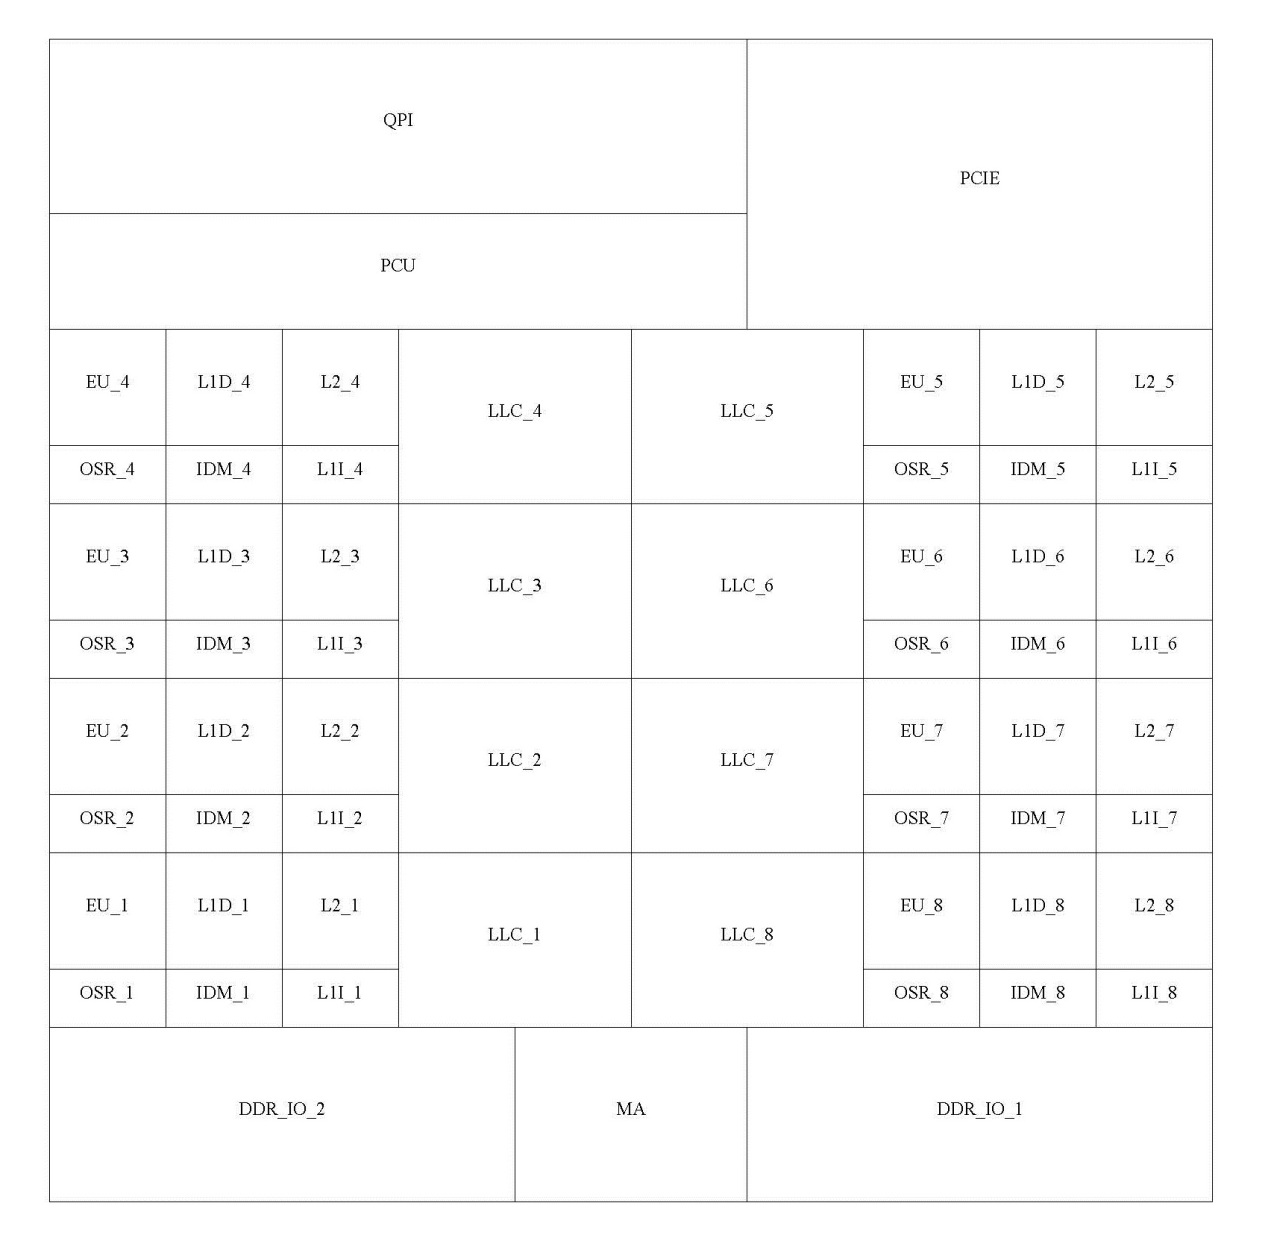
\includegraphics[width=0.8\textwidth,height=0.6\textheight]{Core-i7-3960X}
  \caption{测例二i7-3960X芯片布局}
  \label{fig:core-i7-flp}
\end{figure}

\begin{figure}[H]
  \centering
  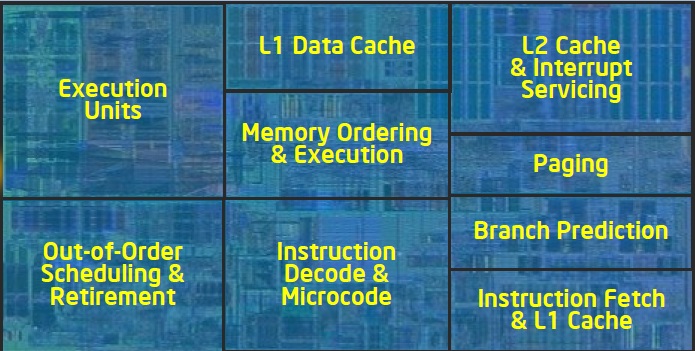
\includegraphics[width=0.9\textwidth,height=0.35\textheight]{InnerCore-Core-i7-3960X}
  \caption{测例二i7-3960X核内的布局}
  \label{fig:inner-core-core-i7-flp}
\end{figure}

对于测例1和测例2,进行类似的实验方案。该方案过程如下:根据表\ref{tab:chap5:exp-flp-parameters}中所示功率参数分配设置方案, 首先重复地随机产生功耗分布;然后,在考虑电热耦合效应的情况下, 分别采用BlockTAM、CoreTAM和BlockInsideCoreTAM方法,获得每个功率分布的温度稳定分布;最后将得到的结果与HotSpot的分析结果进行对比。

测例3基于测例1中采用过的Alpha21264核心,构建多个对于16核的虚拟芯片的布图规划。为了模拟温敏布局规划过程, 本文对各个布图方案进行热分析,在模拟过程中,测试本文方法的运行耗时或效率。

\section{针对MPSoC结构级热分析算法精度的实验数据与分析}
正如前文所提到的,本文按照表\ref{tab:chap5:exp-flp-parameters}中设定的功率参数\onlinecite{MySSTAPaper},随机产生100个功率输入向量; 然后采用HotSpot、BlockTAM、BlockInsideCoreTAM、CoreTAM这4种热分析方法, 测试各个核与功能模块的温度与静态功耗。其中,一个核的静态功耗值等于所属模块的静态功耗值之和, 这个核的局部热点温度是它的Core\_x模块温度。本文以HotSpot的分析结果值作为基准,来计算其余3种方法的相对误差。 由于芯片的工作温度均是相对环境温度$T_{Amb}$而言,所以使用式\ref{equ:chap5:et}来计算温度误差$E_T$:
\begin{equation}
\label{equ:chap5:et}
E_T = |\frac{T-T_{HotSpot}}{T_{HotSpot}-T_{Amb}}|
\end{equation}
其中$T_{HotSpot}$是HotSpot的测值,$T$是本文方法的温度计算值。同时,采用式\ref{equ:chap5:eplk}来计算静态功耗误差$E_{Plk}$:
\begin{equation}
\label{equ:chap5:eplk}
E_{Plk} = |\frac{Plk-Plk_{HotSpot}}{Plk_{HotSpot}}|
\end{equation}
式\ref{equ:chap5:eplk}中$Plk_{HotSpot}$是HotSpot的静态功耗测值,$Plk$是本文方法的静态功耗计算值。

3种方法的温度误差被列入表\ref{tab:chap5:temp-error}\onlinecite{MySSTAPaper}。从表中不难看到,BlockTAM的精度最高,平均误差小于1.6\%, 最大误差小于5\%;BlockInsideCoreTAM的精确效果次之, 平均误差小于4.2\%,最大误差小于15\%;CorTAM的精度最低,平均误差达到33\%,最大误差达到45\%。 所以,BlockTAM和BlockInsideCoreTAM这2种方法均可以提供满意的热分析精度。

3种方法的静态功耗误差如表\ref{tab:chap5:power-leakage-error}所示\onlinecite{MySSTAPaper}。BlockTAM的精度最高,最大误差小于0.5\%; BlockInsideCoreTAM的精度次之, 平均误差小于1.2\%, 最大误差小于3.7\%;CorTAM的精度最低,平均误差达到25\%,最大误差达到35\%。因此,BlockTAM和BlockInsideCoreTAM 2种方法均可以提供满意的静态功耗分析精度。

为了考察本文方法静态功耗与温度分析的误差来源,图\ref{fig:ex1-plk-error}和 图\ref{fig:ex1-temp-error}\onlinecite{MySSTAPaper}给出了本文3种方法对测例1中的各个模块, 所产生的静态功耗与温度相对误差。对本文3种方法的误差分析如下:
\begin{enumerate}[1)]
\item BlockTAM方法的误差分析:由于BlockTAM是根据HotSpot软件的分析结果进行的自下而上的建模, 所以具有与HotSpot软件最近分析精度。如图\ref{fig:ex1-plk-error}所示,各模块的静态功耗分析误差小于0.3\%; 如图\ref{fig:ex1-temp-error}所示,各模块的稳态温度分析误差小于4\%。
\item CorTAM方法的误差分析: 在测例1中的一个核内,具有高功耗(高发热量)的Core\_x模块自然是高温模块,在其总功耗中,静态功耗所占的比例较高; 而其他3个模块(L2\_x、L2\_Left\_x、 L2\_Right\_x)是具有低功耗的低温模块,其静态功耗所占的比例也较低。如图\ref{fig:ex1-plk-error}所示, 产生局部热点的Core\_x模块温度明显高于其他核内模块。CorTAM模型假设核中所有模块的温度均等于核的局部热点温度,这与事实有着较大的出入, 导致其所计算出来的低温模块静态功耗被明显拉高,故而产生了11\%-15\%的较大误差。另一方面来说,高温模块的温度就是核内的局部热点温度, CorTAM所计算出来的高温模块静态功耗也就理所应该较为精确(其相对误差小于2\%)。由于低温模块的静态功耗计算误差明显偏大, 以核内所有模块功耗总和来计算核的局部热点温度就会产生较大的误差; 如图\ref{fig:ex1-temp-error}所示,其所产生的温度误差处于6\%-8\%之间,明显大于其他2种方法。

\item BlockInsideCoreTAM方法的误差分析:该方法正视了核内模块温度之间具有着明显差别,所以,仅仅将核外模块作为一个影响整体进行考虑。 由于仅将热点之间的相关热阻作为核间影响的系数,所以该方法对于热点温度和静态功耗, 可以提供较高的精度(如图\ref{fig:ex1-plk-error}所示,各模块的静态功耗误差小于0.7\%); 但其对于核内低温模块的温度计算精度则较差 (如图\ref{fig:ex1-temp-error}所示,产生热点的高温模块的温度误差小于2.2\%,但低温模块的温度误差则达到了5\%-11\%)。
\end{enumerate}

\begin{table}
\centering
\caption{本文测例各功能模块的面积与功耗参数设定}
\begin{tabular}{c c c c}
\hline\hline
测例 & 功能模块 & 面积($mm \times mm$) & 动态功率($w$) \\
\hline
 & Core\_x & $3\times 3$ & 10-20 \\

 & L2\_left\_x & $5\times 3$ & 1-2.5 \\
\raisebox{1.5ex}{1}
 & L2\_x & $5\times 5$ & 2-5 \\
 & L2\_right\_x & $3\times 5$ & 1-2.5 \\
\hline
 & DDR\_IO\_2 & $3 \times 8$ & 2-6.5 \\
 & MA & $3 \times 4$ & 2-6.5 \\
 & DDR\_IO\_1 & $3 \times 8$ & 2-4.5 \\
 & OSR\_x & $1 \times 2$ & 0-1 \\
 & IDM\_x & $1 \times 2$ & 0-1 \\
 & L1I\_x & $1 \times 2$ & 0-2 \\
2 & EU\_x & $2 \times 2$ & 1-8 \\
 & L1D\_x & $2 \times 2$ & 0.5-3 \\
 & L2\_x & $2 \times 2$ & 0.5-4.5 \\
 & LLC\_x & $4 \times 3$ & 2-6.5 \\
 & PCU & $2 \times 8$ & 2-7.5 \\
 & QPI & $3 \times 12$ & 2-7.5 \\
 & PCIE & $3 \times 8$ & 2-7.5 \\
\hline
\end{tabular}
\label{tab:chap5:exp-flp-parameters}
\end{table}


\begin{table}
\centering
\caption{多核芯片核内局部热点的温度计算误差对比}
\begin{tabular}{c c c c c c c}
\hline\hline
 & \multicolumn{2}{c}{BlockTAM} & \multicolumn{2}{c}{CoreTAM} & \multicolumn{2}{c}{BlockInsideCoreTAM} \\
 & Avr.$E_T$ & Max.$E_T$ & Avr.$E_T$ & Max.$E_T$ & Avr.$E_T$ & Max.$E_T$ \\
 \hline
测例1 & 1.361\% & 1.574\% & 6.573\% & 12.851\% & 2.223\% & 2.259\% \\
\hline
测例2 & 1.447\% & 4.864\% & 33.063\% & 45.840\% & 4.185\% & 14.598\% \\
\hline
\end{tabular}
\label{tab:chap5:temp-error}
\end{table}

\begin{table}
\centering
\caption{多核芯片各核静态功耗的计算误差对比}
\begin{tabular}{c c c c c c c}
\hline\hline
 & \multicolumn{2}{c}{BlockTAM} & \multicolumn{2}{c}{CoreTAM} & \multicolumn{2}{c}{BlockInsideCoreTAM} \\
 & Avr.$E_{Plk}$ & Max.$E_{Plk}$ & Avr.$E_{Plk}$ & Max.$E_{Plk}$ & Avr.$E_{Plk}$ & Max.$E_{Plk}$ \\
\hline
测例1 & 0.314\% & 0.327\% & 6.857\% & 10.816\% & 0.495\% & 0.570\% \\
\hline
测例2 & 0.144\% & 0.317\% & 25.123\% & 35.084\% & 1.196\% & 3.687\% \\
\hline
\end{tabular}
\label{tab:chap5:power-leakage-error}
\end{table}

\begin{table}
\centering
\caption{1000组热分析各算法计算耗时及加速倍数$X$对比}
\begin{tabular}{c c c c c}
\hline\hline
分析算法 & HotSpot & BlockTAM & CoreTAM & BlockInsideCoreTAM \\ [0.5ex]
\hline
$T_{Anls}/s$ & 61.301 & 1.216 & 0.414 & 0.927 \\
\hline
$T_{Totl}/s$ & 61.301 & 4.663 & 4.374 & 4.374 \\
\hline
$X_{Anls}$ & BASE & 50.416 & 147.962 & 66.100 \\
\hline
$X_{Totl}$ & BASE & 13.147 & 15.876 & 14.014 \\
\hline
\end{tabular}
\label{tab:chap5:time-speedup}
\end{table}

\begin{figure}[H]
  \centering
  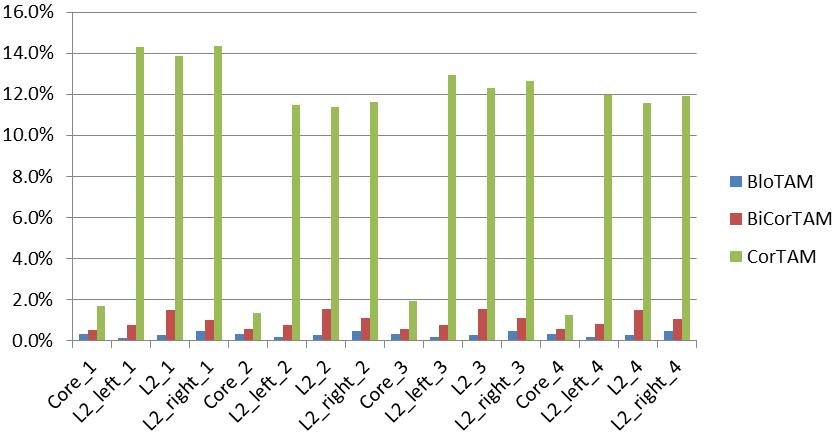
\includegraphics[width=0.8\textwidth,height=0.32\textheight]{EX1-PLK-ERROR}
  \caption{对测例1中各模块的静态功耗计算误差}
  \label{fig:ex1-plk-error}
\end{figure}
\begin{figure}[H]
  \centering
  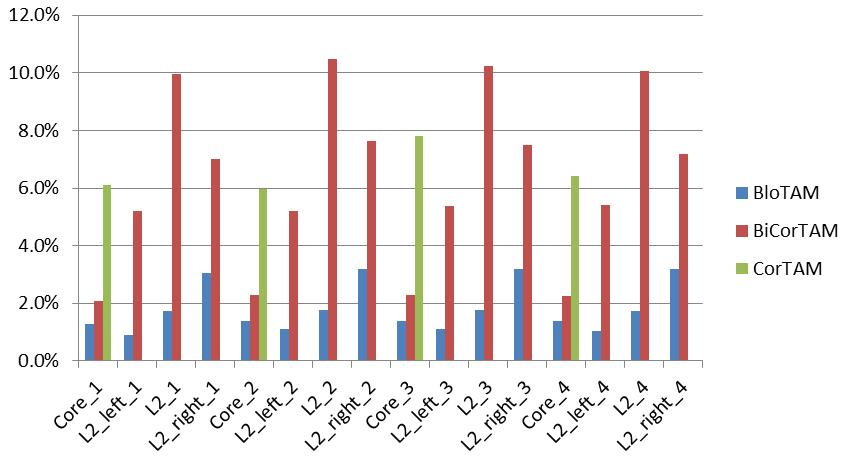
\includegraphics[width=0.8\textwidth,height=0.32\textheight]{EX1-TEMP-ERROR}
  \caption{对测例1中各能模块峰值温度的计算误差}
  \label{fig:ex1-temp-error}
\end{figure}


\section{针对MPSoC结构级热分析算法速度的实验数据与分析}
\label{exp-speedup}
本文采用16核的测例3(大测例)对其进行计算速度的验证。3种方法需要采用HotSpot软件对相关热阻的参数提取, 由于芯片中有16个核、每核有4个模块, 所以本文方法需要进行64次HotSpot模拟,这部分耗时被称为建模时间$T_{Model}$。

实验测试结果表明,$T_{Model} = 3.447$ 秒(S)。建模之后,本文方法基于这些参数,采用式\ref{equ:chap4:blotam-tii}、\ref{equ:chap4:cortam-tpp}、式\ref{equ:chap4:bicortam-tii} 对1000个输入功耗进行温度分析与静态功耗计算,这部分耗时被称为热分析时间$T_{Anls}$; 建模时间与热分析时间两部分的总和被称为总耗时$T_{Totl}=T_{Model}+T_{Anls}$。 本文方法所提供的加速倍数$X$是HotSpot的耗时与本文方法耗时之比,其中, 不计入建模时间而只计入热分析计算耗时的加速比被称为热分析加速倍数$X_{Anls}$, 而总耗时加速倍数为$X_{Totl}$。

表\ref{tab:chap5:time-speedup}列出了耗时与各种加速比的计算结果。可以看出,本文方法的总耗时主要一部分是建模时间消耗; 只要提取出了模型参数, 由于本文的模型复杂度很低,采用式\ref{equ:chap4:blotam-tii}、 \ref{equ:chap4:cortam-tpp}、式\ref{equ:chap4:bicortam-tii} 计算温度与静态功耗就是一个非常快速的计算过程(即$T_{Anls}$非常小, 只占$T_{Totl}$很小的部分)。 与HotSpot软件相比,本文3种方法分析计算的加速比$X_{Anls}$分别达到50、147、和66; 但考虑到$T_{Anls}$只占$T_{Totl}$很小的部分,所以本文3种方法总耗时的加速比只能达到13、15、和14。

从表\ref{tab:chap5:temp-error}-表\ref{tab:chap5:time-speedup}的算法精度与复杂度的比较结果\onlinecite{MySSTAPaper}可以看出: 与HotSpot软件相比, 本文的BlockTAM和BlockInsideCoreTAM在满足精度要求的前提下(热点温度误差小于2.2\%), 获得了满意的加速效果,总耗时的可以达到13倍和14倍的加速效果。

\section{小结}
第\ref{cha:SSTA}章中,采用自下而上的建模方法对MPSoC结构级热分析方法进行了探索,同时提出了3种具有不同算法复杂度与精度的热分析方法: 模块级方法、核级方法与考虑本核内模块相互影响的改良核级方法。 这三种算法之所以能在保证分析计算精度的前提下、 获得比较好的加速效果,归根结底是因为对整个芯片的热分析模型从结构级进行了合理适度的等效简化。
本章对第\ref{cha:SSTA}章中所提出的各种算法进行了大量的实验验证。实验数据数据表明: 对核数较多MPSoC进行热分析的时候,BlockTAM和BlockInsideCoreTAM均具有算法复杂度低和精度高的优点: 平均相对增量误差最大不超过3\%,同时可以获得14倍左右的运算加速效果。 